%\documentclass{article}
\documentclass[11pt,copyright]{fsuthesis}

% Language setting
% Replace `english' with e.g. `spanish' to change the document language
\usepackage[english]{babel}
\addto\captionsenglish{\renewcommand*{\contentsname}{Table of Contents}}

% Set page size and margins
% Replace `letterpaper' with `a4paper' for UK/EU standard size
%\usepackage[letterpaper,top=2cm,bottom=2cm,left=3cm,right=3cm,marginparwidth=1.75cm]{geometry}

% Useful packages
\usepackage[colorlinks=true, allcolors=blue]{hyperref}
\usepackage{amsmath,amsthm,amssymb}
\usepackage{mhchem}
\usepackage{graphicx}
\graphicspath{{figures/}}
\usepackage{verbatim}
\usepackage{pgfplots}
\usepackage{csquotes}

\usepackage[backend=biber, style=numeric]{biblatex}
\addbibresource{source.bib}

\title{INVESTIGATIONS OF NUCLEAR STRUCTURE IN MASS-9 SYSTEMS USING NEUTRON SPECTROSCOPY}
\author{Matthew Gerard Mestayer II}
\college{Florida State University}
\department{Physics Department}
\manuscripttype{Dissertation}
\degree{PhD}
\degreeyear{2026}
\defensedate{April 27, 2026}

\committeeperson{Sergio Almaraz-Calderon}{Thesis Director}
\committeeperson{Ingo Widenhover}{Committee Member}
\committeeperson{Kevin Fossez}{Committee Member}
\committeeperson{Rachel Yohay}{Committee Member}
\committeeperson{Anke Meyer-Baese}{Committee Member}

\clubpenalty=9999
\widowpenalty=9999
\pgfplotsset{compat=1.18}

\begin{document}

\frontmatter
\maketitle
\makecommitteepage

\tableofcontents

\begin{abstract}
%Mirror nuclei present a rich ground for testing isospin-symmetry breaking effects, especially the mass-9 isospin systems due to their deviations from the Isobaric Mass Multiplet Equation.
Mirror nuclei present a rich ground for testing isospin-symmetry breaking effects, especially the mass-9 isospin systems due to the proximity of certain states to particle separation thresholds. In particular, an observation of the $\frac{1}{2}+$ state in $^9$B would serve as a probe of Thomas-Ehrman effects in this system due to the ambiguous direction and magnitude of the shift. Characterizations of this state have been largely unsuccessful due to the relative proximity of large resonances. To observe this state, the $^7Li(^3He,n)$ reaction is used. The neutrons from this reaction are detected by the liquid scintillator array CATRiNA. Current work done to observe this state is detailed below. Improvements and future plans are also listed. 
\end{abstract}

\mainmatter

\chapter{Introduction}

\section{Motivation}

The precise characterization of the nucleon-nucleon interaction is an ongoing endevour in nuclear physics. A degree of freedom associated with this interaction isospin. Under the formalism describing isopsin, protons and neutrons both have total isospin $T=\frac{1}{2}$. Similar to intrinsic spin, the isospin z-projection $T_z$ takes the values $\mp\frac{1}{2}$ for protons and neutrons respectively. Historically, isospin was derived from W. Heisenberg's attempt to treat both protons and neutrons as two states of the same particle, which was expanded upon by E. Wigner and given the name 'isotopic spin' as a means of listing the emergent symmetries of strongly-interacting nuclear systems \cite{wigner1937consequences}. In particular, from this 'isotopic spin', or isospin, Isobaric Analog States (IAS) can be defined, which are nuclear states with equivalent isospin $T$ but differing $T_z$ values. From just the strong interaction, IAS would have equivalent energy levels. Due to the presence of Coulomb interactions from proton-proton repulsion, the isospin symmetry between IAS is broken, giving rise to differences in energy levels \cite{zelevinsky2017physics}. The contributions to these energy shifts arise from various admixtures of interactions within the nucleus.
\\ \\
An contribution to this energy shift that can occur in nuclei is the Thomas-Ehrman shift (TES), an energy shift between the energy states in mirror nuclei from higher-order Coulomb interactions. Initially proposed by J. Ehrman and R. Thomas to describe the displacement in the first excited states between $C^{13}$ and $N^{13}$ \cite{ehrman1951displacement}\cite{thomas1952analysis}, this shift is attributed to the interaction between nuclei structured as a core and valence nucleon in which single-particle valence proton wavefunctions become spacially extended thus driving down the measured energies relative to the energies of the neutron-rich member. The TES is usually more pronounced in states with a weak centrifugal barrier and can be influenced by continuum effects. In particular, coupling to the continuum can induce a separate shift which can lead to an inverted TES, where the energies of the proton-rich member are greater than the neutron-rich member. The mirror-pair ${^9B}$ and ${^9Be}$ offers an ideal testing ground for these contributions due to their low mass, closeness of $^9$B to the particle separation threshold, and ambiguity of the direction of the TES for the $\frac{1}{2}+$ state in $^9$B. 
\\ \\
To fully determine the shift between energy levels between the mirror pair $^9$Be - $^9$B, a proper observation of the $\frac{1}{2}+$ state within $^9$B is required. %The corresponding state within $^9$Be at 1.68 MeV has been well-studied due to the state being above the neutron separation energy at 1.66 MeV. 
The corresponding state within $^9$Be at 1.68 MeV has been well-studied due to the state having a relatively narrow width at 214 keV. However, the $\frac{1}{2}+$ state for $^9$B has a proton separation energy of -186 keV \cite{Wang_2012}, meaning that all states exist as resonances and are prone to experience a large degree of continuum. A decisive measurement of this state would confirm if the magnitude of the TES, along with demonstration a normal or inverted TES, setting an important benchmark for any model attempting to explain low-mass nuclei. 
\\ \\
Various measurements of the $\frac{1}{2}+$ state in $^9$B have been made, with limited success. After the first official report in 1955 \cite{PhysRev.100.91}, other authors have attempted to characterize this state. Historically, two different values have been proposed for this state. In 1962, G. Symons measured the state at 1.7(2) MeV\cite{SYMONS1962175}, which would be contrasted with M. Tiede, who found that the state seemingly split into values of 0.8 and 1.8 MeV \cite{PhysRevC.52.1315}. Unsuccessful searches have continued; however, certain promising developments have recently occured. An solution to the apparent bifurcation of the $\frac{1}{2}+$ state was determined by A. Brooks et al., who proposed a "ghost peak" due to leakage of the ground state, appearing near 0.8 MeV. This would be followed by another paper in which a resonance was characterized with an energy of $1.83(5) MeV$ and intrinsic width of $850^{110}_{88} keV$. However, this characterization could not unambiguously confirm this state as a $\frac{1}{2}+$ state since angular distributions could not be extracted \cite{5rny-7zbk}. Further work is required to properly characterize this state. 
\\ \\

\begin{figure}[h!]
  \centering
  \includegraphics[width=0.6\textwidth]{k_gul_data.png}
  \caption{Various ToF spectra taken by K. Gul with different bombardment energies.}
  \label{fig:kgulspec}
\end{figure}

In characterizing the $\frac{1}{2}+$ of $^9$B, the $(^3He,n)$ reaction has met with mixed success. There have been studies into the structure of $^9$B using this reaction, starting in 1965 with Dietrich's investigation using time-of-flight spectroscopy using a plastic scintillator for neutron measurement. Highly excited states in $^9$B where measured at 12.06, 14.01, 14.67, and 16.04 MeV, along with an assignment of $T=\frac{3}{2}$ for the 14.67 MeV state, though no low lying states could be resolved \cite{DIETRICH196549}. The next work that found a potential $\frac{1}{2}+$ state was performed by K. Gul et al. Low lying states, such as the ground state, 2.345, 2.78, and 4.8 were identified, along with a peak between the ground state and the 2.33 state. However, this peak was attributed to a two-stage process of populating the 11.82 MeV state in $^9$Be using $(^3He,p)$, followed by a neutron decay of $^9$Be to $^8Be$ \cite{gul197018o}. After this work, no other study would make an explicit attempt to measure the $\frac{1}{2}+$ state using the $(^3He,n)$ reaction. A modern characteriation of this state using the $(^3He, n)$ reaction is needed.
\\ \\
The masses of nuclei within an isobaric multiplet are described by the Isobaric Multiplet Mass Equation (IMME): \\
\[
M(T_z)=a(\alpha,T_z) + b(\alpha,T_z)T_z + c(\alpha,T_z)T_z^2 \] \\
where $\alpha$ refers to any other relevant quantum numbers besides the isospin and the z-projection. In order to validate this equation, a $T=\frac{3}{2}$ multiplet is needed. In order to determine the coefficients of this equation, a fit to the mass excess for the nucleus in question is required, usually deduced from a measurement of Q-value \cite{PhysRevLett.25.530}. A multiplet known to significantly deviate from this equation is the A = 9 $T=\frac{3}{2}$ quartet, involving $T=\frac{3}{2}$ states in $^9Li$, $^9$Be, $^9$B, and $^9C$. To describe this quartet, a cubic term $dT_z^3$ is needed in the IMME to obtain agreement. The physical interpretation, along with the magnitude, of this cubic term is a point of contention. A recent evaluation found a coefficient of $d=6.7 \pm 1.5 keV$ was required to ensure agreement with known mass excesses \cite{maccormick2014evaluated}. The physical reason for this term has been attributed to multiple explainations, from the radial extent of the least-bound proton in $^9C$ \cite{bertsch1970tz3} to isospin-mixing \cite{brodeur2012elucidation}. A more precise measurement of highly excited states within $^9$B, along with a characterization of the isospin-mixing strengths for various states, is necessary to resolve this discrepancy. 

\begin{figure}[h!]
  \centering
  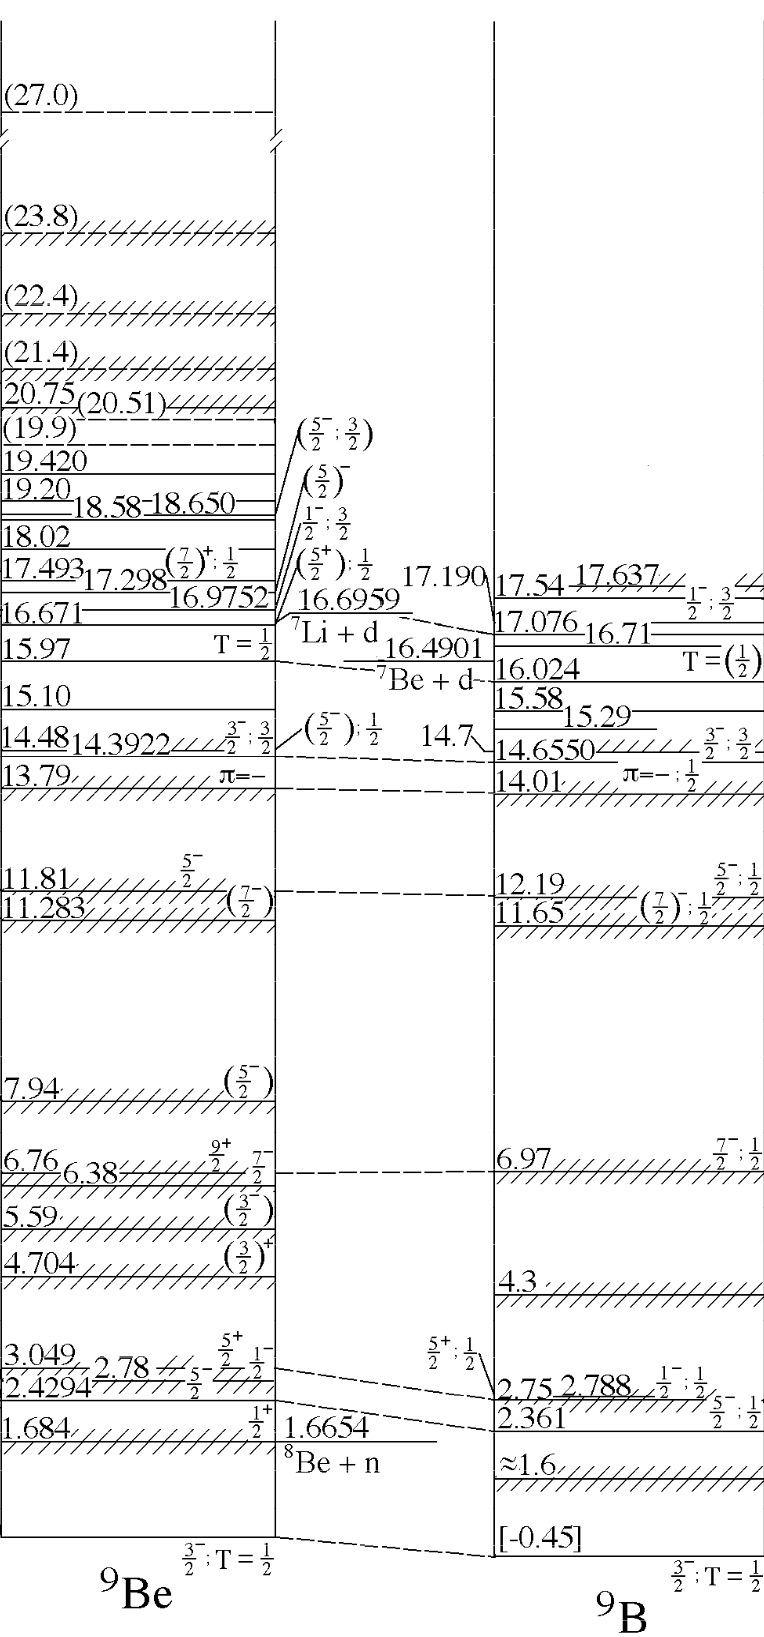
\includegraphics[width=0.6\textwidth]{mass_9.png}
  \caption{}
  \label{fig:mass9}
\end{figure}

\chapter{Reaction Kinematics}

The reaction ($^3$He, n) is used to probe states in $^9$B. The measurement of neutron energy spectra to deduce information about nuclei is neutron spectroscopy. A technique for measuring this spectrum is time-of-flight (ToF) spectroscopy. ToF spectroscopy works by measuring the flight time of the neutron from the target to the detector. In practice, this is usually done with by taking the difference of the measured neutron flight time with respect to a reference signal. In the work described by this prospectus, the signal is an RF signal pulsed at 82.5 ns. The neutron's flight time is inversely proportional to its energy since the neutron is massive. This dependence on energy allows for the separation of neutron groups corresponding to populated excited states. 

The nuclear reaction used by the work described by this prospectus is a transfer reactions. A transfer reaction is a nuclear reaction in which an incident nucleus collides with another nucleus, transferring nucleons. This involves a projectile nucleus, typically a light nucleus that has some energy with respect to the lab frame and a target nucleus that is at rest. The projectile interacts with the target, which results in a residual nucleus and an ejected nucleus, or ejectile, that travels outwards and interacts with a detector, resulting in a signal that contains information about the ejected particle. In this prospectus, this type of reaction will be represented as $A(a,b)B$, where a is the projectile, A is the target, B is the residual, and b is the ejectile. This reaction describes a transfer reaction, in which the interaction involves a transfer of nucleons between the projectile and target nucleus, and is the primary means used to populate states in $^9$B in this prospectus. In this case, the reaction is $^7Li(^3He,n)^9B$. Using this reaction, a measurement of the resulting ejectile yields information of the populated $^9$B state from on kinematics. In our case, this ejectile is simply a neutron. \\ 

An observed quantity useful in describing nuclear kinematics is the Q-value. The Q-value is defined as the difference in mass energy between the incoming particles and  outgoing particles for a given reaction or \\ \[Q = (m_a + m_A - m_b - m_B)c^2 (1).\] \\ In order to excite the residual nucleus to an excited state, extra energy is needed to change the populated state of the residual nucleus. For a Q-value corresponding to the population of an excited state $Q$, the excitation energy of the residual nucleus can be written as \\ \[Q = Q_0 - E_{ex} (2)\] \\ where $Q_0$ is the Q-value of the ground state reaction and $E_ex$ is the residual nucleus excitation energy.

\begin{figure}[h!]
  \centering
  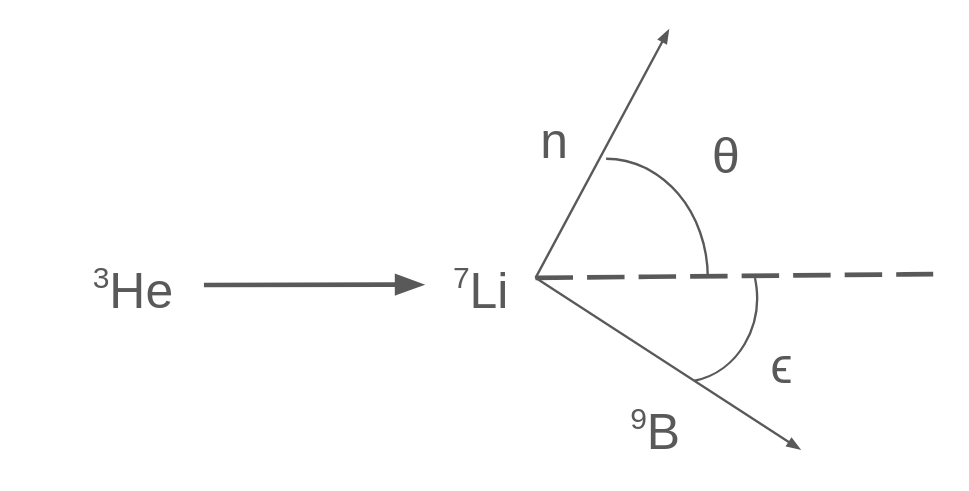
\includegraphics[width=0.6\textwidth]{kinematics.png}
  \caption{Figure 2.1: Kinematic representation of transfer reaction. The $^3$He nucleus is the projectile, the $^7$Li nucleus is the target, the $^9$B nucleus is the residual, and the neutron (n) is the ejectile.}
  \label{fig:Kinematics}
\end{figure}

%\begin{comment}
To derive the energies populated by the residual nucleus from the ejectile, one applies conservation of momentum $p$ and energy $E$\\
\\
\begin{equation}
p_a+p_A=p_b+p_B (3) \end{equation}
\begin{equation}
E_a+E_A=E_b+E_B. (4)
\end{equation}\\

Using the known energy relation $E = \frac{p^2}{2m} + mc^2 (4)$ along with (1), (2), (3), and (4), the excited states of the residual nucleus with respect to reconstructed neutron energy is 
\begin{comment}
where $E = \frac{p^2}{2m}+mc^2$. The conservation of momentum can be written as \\
\begin{equation}
p_a=p_bcos\theta+p_Bcos\epsilon  (3) \end{equation}
\begin{equation}
0=p_bsin\theta+p_Bsin\epsilon (4). 
\end{equation}
\\
Using $p=\sqrt{2mT}$ with kinetic energy $T$ and substituting (4) into (3), we have \\
\[T_B = \frac{1}{m_B}[m_aT_a+m_bT_b-2\sqrt{m_am_bT_aT_b}cos\theta].\] 
Going further, we can take the Q-value, or the difference in mass energy between the initial and final nuclei, which is given as \\
\[Q=(m_a+m_A-m_b-m_B)c^2.\]
Using (1) and rearranging with $E=T+\frac{p^2}{2m}$,\\
\[Q = (m_a-m_b-m_c)c^2=T_b-T_a+T_b=T_b-T_a+\frac{1}{m_B}[m_aT_a+m_bT_b-2\sqrt{m_am_bT_aT_b}cos\theta].\]\\
The excitation of the residual nucleus can then be expressed as\\\[Q = Q_0-E_{ex} (5),\]\\
where $Q_0$ is the Q-value of the ground state in $^9$B and $E_{ex}$ is the excitation energy of the nucleus.
\[E_{ex} = Q_0 - (m_a+m_A-m_b-m_B)c^2=Q_0-T_b-T_a+T_B \]
\\
\[=Q_0-T_b-T_a+\frac{1}{m_B}[m_aT_a+m_bT_b-2\sqrt{m_am_bT_aT_b}cos\theta]\].
\\ 
\end{comment}
\[E_{ex} = =Q_0-T_b-T_a+\frac{1}{m_B}[m_aT_a+m_bT_b-2\sqrt{m_am_bT_aT_b}cos\theta] \]
\\
where $T_b$ and $m_b$ are ejectile kinetic energy and mass, $T_a$ and $m_a$ are projectile kinetic energy and mass, $m_B$ is the residual nucleus energy, $\theta$ is the angle at which the ejectile leaves the reaction in the lab frame, and $Q_0$ is the ejectile ground state Q-value. 

\newpage

States in nuclei are further characterized by their total spin $J$ and their parity $\Pi$. This $J^{\Pi}$ value features within angular distribution plots that plot the differential cross section $\frac{d\sigma}{d\Omega}$ over the center of mass angle $\theta_{cm}$. The differential cross section is a measure of the likelihood of a given reaction occurring as a function of the angular distribution of thereaction products. In order to compute this angular distribution, we use the equation \\ \\$\frac{d\sigma}{d\Omega}=\frac{N}{\epsilon \rho I d\Omega}$ \\ \\where $N$ is the number of ejectile nuclei detected, $\epsilon$ is the detector efficiency, $\rho$ is the atomic density of the target, $I$ is the number of projectile nuclei incident to the target, $d\Omega$ is the solid angle of the detector. These experimentally determined angular distributions can then be compared to theoretical angular distributions using the Distorted Wave Born Approximation (DWBA) and optical model to find spectroscopic factors, denoted as $C^2S$. The experimental and theoretical angular distributions are related by \\ \\$(\frac{d\sigma}{d\Omega})_{experiment}=C^2S(\frac{d\sigma}{d\Omega})_{theory}$.

\begin{figure}[h!]
  \centering
  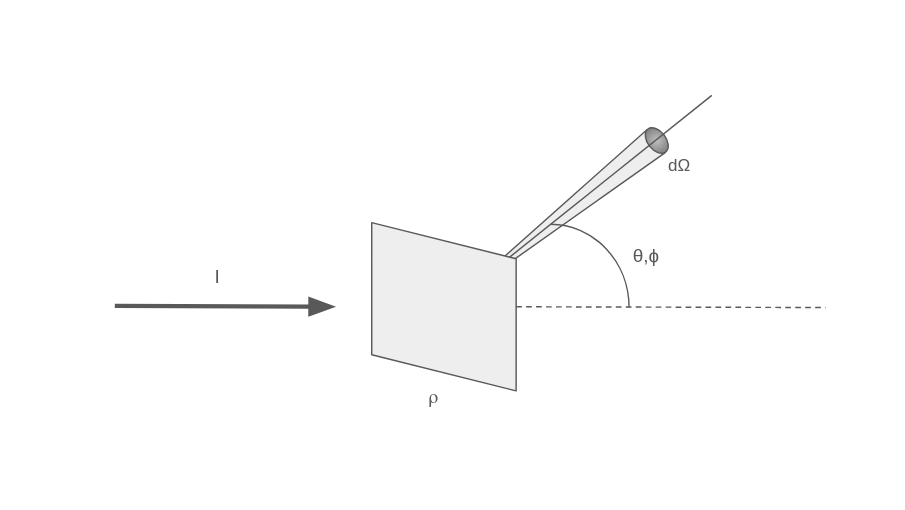
\includegraphics[width=0.6\textwidth]{xcschematic.png}
  \caption{Figure 2.2: Visual example of kinematics in cross section calculation.}
  \label{fig:Cross Section Model}
\end{figure}

\chapter{CATRiNA}

\section{CATRiNA}

In order to detect particles such as a neutron, which primarily interact via elastic scattering, scintillators are used.  A scintillator refers to any material that emits light after interacting with radiation. This light can then be converted into an electric signal via a Photomultiplier Tube (PMT) \cite{knoll2010radiation}.
\\ \\
The Compound Array for Transfer Reactions in Nuclear Astrophysics (CATRiNA) is an array of deuterated benzene scintillators. The scintillators are stored in a cylindrical container with two sizes: 4"x2" and 2"x2". The scintillator material is the EJ-315 deuterated liquid scintillator produced by Eljen Technology. The coupled Photomultiplier Tube (PMT) is the 9821B PMT developed by ET Enterprises for the 4"x2" scintillator and the Hamamatsu R7724 PMT for the 2"x2" scintillator \cite{ej315info} \cite{4x2pmtinfo} \cite{2x2pmtinfo}. Both scintillators rely on the scintillation of deuterated benzene to accurately measure incoming neutron energies. The scintillating molecule, benzene, comprises a hexagon of carbon atoms with a deuterium atom bonded to each carbon atom. Two or three of the valence electrons of each carbon atom occupy the $\sigma$ orbital in between the carbon and deuterium atoms and are strongly localized. The remaining electrons occupy the $\pi$ orbitals, which extend outside of the molecular plane and are not strongly localized \cite{BROOKS1979477}. Transitions between the $\pi$ orbital electrons are responsible for the luminescence seen within the deuterated benzene. The electrons can be excited into either singlet or triplet states as shown in Figure 3.1. 
%Only transitions between levels emit gamma radiation. Transitions between vibrational states within the same level thermally de-excite. 
From these excitations, there are three principal decays that can occur to excited $\pi$ orbital electrons. 
\\ \\
Prompt fluorescence is the process by which an electron, excited into a singlet state, decays into the ground state. This transition is short lived, with a half-life of a few ns \cite{leo1994techniques}. Phosphorescence refers to a process where a singlet electronic configuration is converted into a triplet configuration via inter-system crossing.  
%Since the triplet has a much longer lifetime than the singlet with up to $10^{-3}$ s, this results in a delayed form of emission. Since the triplet state is at a lower energy relative to the singlet state, the emitted photon will have a longer wavelength than fluorescence photons. 
Delayed fluorescence refers to the process where a singlet state, converted into a triplet state, converts back into a singlet state before decaying via fluorescence. The intensity of the fluorescence decays can be represented by the $I = Ae^{-t/\tau_f} + Be^{-t/\tau_t}$, where $\tau_s$ and $\tau_f$ refers to the mean lifetimes of the slow and fast components of the emission spectrum (delayed fluorescence and fluorescence) and $A$ and $B$ corresponds to the relative magnitude of each component. 
\begin{figure}[h!]
  \centering
  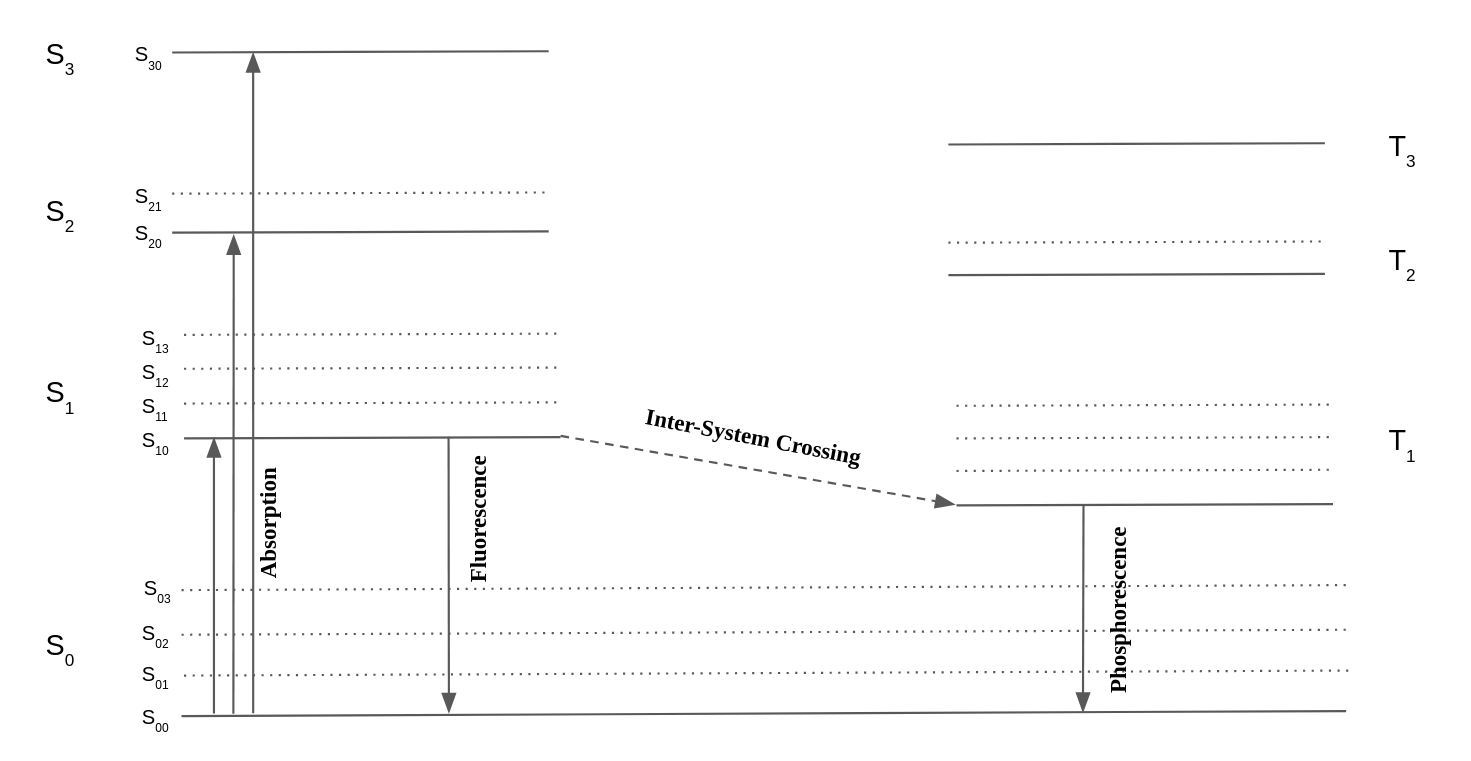
\includegraphics[width=0.6\textwidth]{OrganicLevelScheme.png} 
  \caption{Figure 3.1: A diagram demonstrating a level scheme for a valence electron of carbon. Singlet and triplet states are labelled as $S_i$ and $T_i$ respectively. The dashed lines represent vibration excited states. The black arrows are drawn as a guide of the possible excitations and decays of the electron.} 
  \label{fig:levels_o_scin}
\end{figure}
\\ \\
These two decays are basis of the Pulse-Shape Discrimination (PSD) technique for separating n-$\gamma$ events. The relative magnitude of each component of the emission spectrum is dependent upon the type of incident radiation. $\gamma$ radiation typically has a strong prompt fluorescence component but a small delayed fluorescence component. Neutron radiation has a smaller prompt fluorescence component but a larger delayed fluorescence component. This is because the rate of energy loss within the scintillator $\frac{dE}{dx}$ induces greater amounts of intermolecular interactions, resulting in higher frequencies of delayed fluorescence \cite{leo1994techniques}. This allows for the discrimination of these events via timing gates. As shown in Figure 3.2, the long gate is the total integral of the signal while the short gate is an integral over the rise time. The tail gate, or the difference between the long and short gate integral values, can then be defined. This "tail integral" is consistently greater for neutron-induced events than $\gamma$-induced events, resulting in a PSD spectrum where each tail corresponds to a different radiation type \cite{knoll2010radiation}. 
\\ 
\begin{figure}[h!]
  \centering
  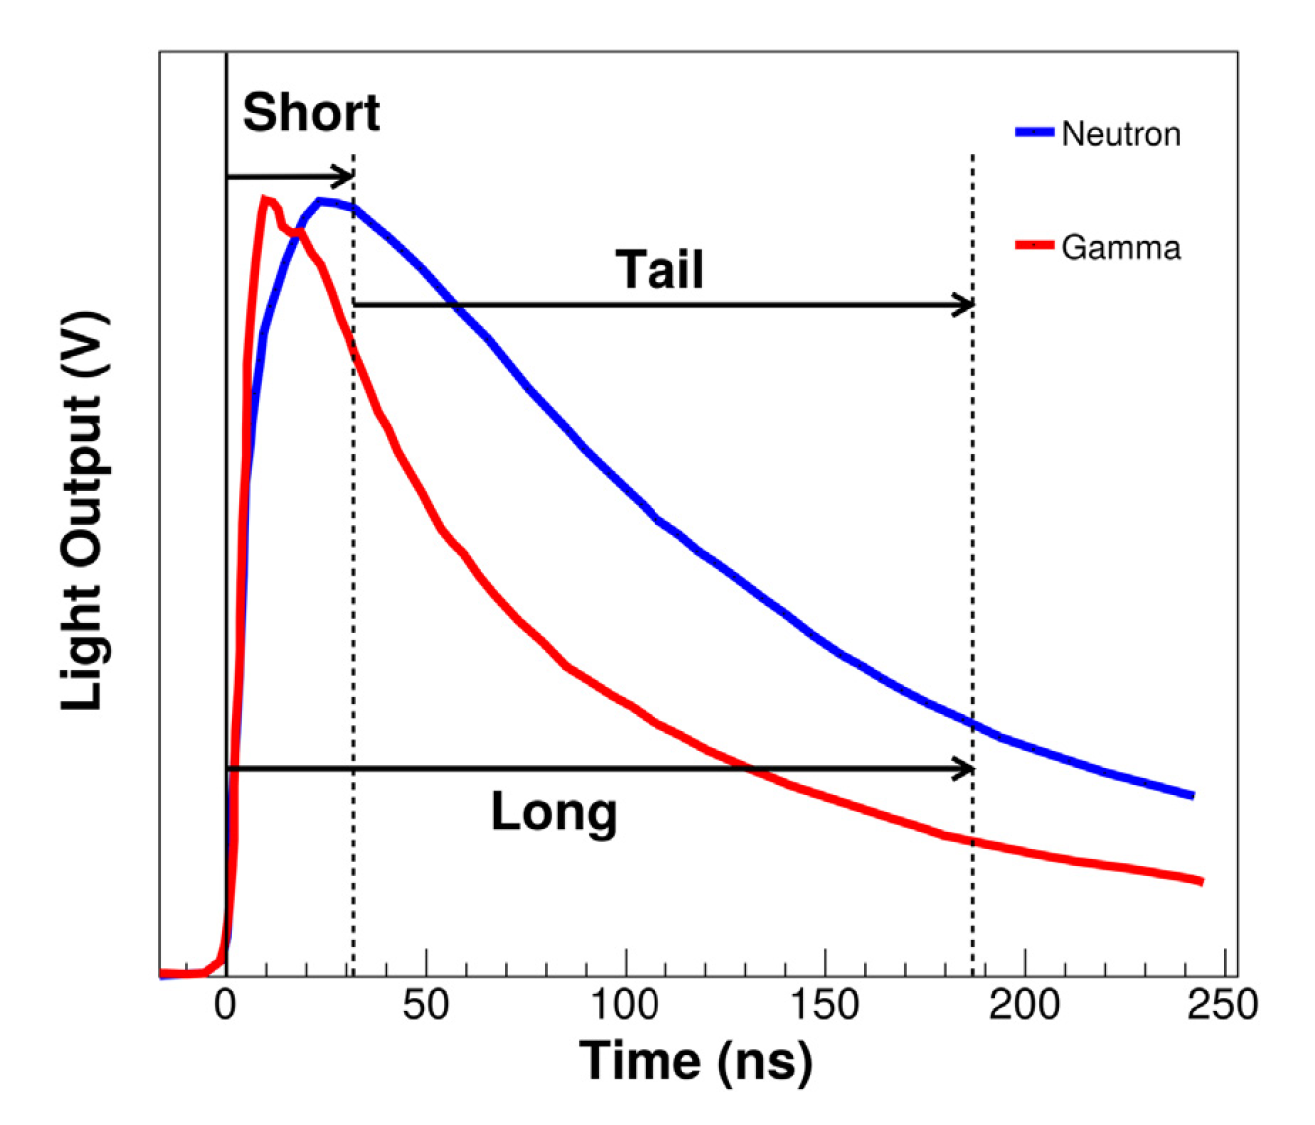
\includegraphics[width=0.6\textwidth]{psd_gate_ex.png}
  \caption{Figure 3.2: From \cite{perello2019characterization}, this plot is an example of gates applied to two waveforms representing an arbitrary $\gamma$ and neutron event compiled in a previous characterization of CATRiNA. Notice the strength of the neutron signal after the short gate relative to the $\gamma$ signal.} 
  \label{fig:psd_gate_ex} 
\end{figure}
\\
Referring to the light-output incident radiation emits when interacting with scintillators, it is customary to define the unit electron-volt electron equivalent, or eVee. An eVee is defined as the light-output an electron with 1 eV of energy gives off. The PSD spectra obtained in this prospectus are plotted in terms of keVee and PSD ratio. The light-output for a given neutron energy is given by \cite{LAWRENCE201321} \\ \[L=aE_{dep}-b(1-e^{-cE_{dep}})\] \\ where a, b, and c are parameters that must be experimentally characterized. From a previous characterization, the results are listed below \cite{morelock2022characterization}. 

\begin{centering}
\begin{tabular}{|c|c|}
  \hline
  4" x 2" detector & 2" x 2" detector \\
  \hline
  0.6109 & 0.6193 \\
  1.946  & 2.036  \\
  0.2625 & 0.2592 \\
  \hline
\end{tabular}
\end{centering}

These parameters allow for the extraction of neutron energies based on light output.

\chapter{Current Work}
\section{08/26/24}

An experiment was run from 08/19/24 to 08/26/24 populating states in $^9$B with the $^7Li(^3He,n)^9B$ reaction. This was achieved with the FN Tandem accelerator at the FSU John D. Fox lab. The $^3He$ beam has an energy of 7 MeV in  the laboratory frame. This was the lowest possible beam energy the Tandem accelerator could coherently transmit the $^3He$ beam. The beam energy was minimized to reduce the resulting neutron energies, int turn increasing the ToF for various neutron groups to achieve greater separation between populated states.
\\ \\
The CATRiNA detectors were placed at backwards angles to further reduce neutron energy. There were three neutron detectors placed at forward angles. All detectors except for the forward detectors were placed at 2 meters from the target ladder. This was done to ensure the anticipated neutron groups would be suitably separated within the ToF spectrum. A beam stop located 3.99 meters after the target ladder was used to halt the beam. Despite using all available shielding, a significant beamstop-induced neutron background was observed within the ToF spectra. The backwards detector angles were located from 97 to 140 degrees. The forwards detector angles were 47 to 50 degrees. 
\\ \\
The $^3$He beam used in this experiment was incident to a target ladder containing three $^7$Li targets, one blank target, one $^{12}$C target, and one phosphor target. The $^7$Li andd $^{12}$C targets had a thickness of 200 and 100 $\mu g/cm^2$. To prevent the oxidation of the $^7$Li targets, the target ladder had to be mounted under vacuum. To reduce unwanted reactions of the beam with the target frame, the phosphor target was used to align the beam due with its luminescence in response to incident radiation. The $^{12}$C target was used to populate the ground state of $^{14}$O via the $^{12}C(^3He,n)^{14}O$ reaction. This resulted in a single neutron group being visible the resulting excitation spectrum. The presence of this peak allowed for corrections to be applied to the angular displacements and distances of the CATRiNA detectors. The Q-value of this reaction is -1.15 MeV, which can be seen as a sharp peak in the figure below. The sharpness of this peak results from the ground state of $^{14}$O having a half-life of 70.6 s, which results in a narrow resonance width. Using this correction, information regarding the populated states in $^{9}B$ where extracted. The plots regarding the $^{12}$C($^3$He,n)$^{14}$O reaction can be seen below. 

\begin{figure}[h!]
  %\centering
  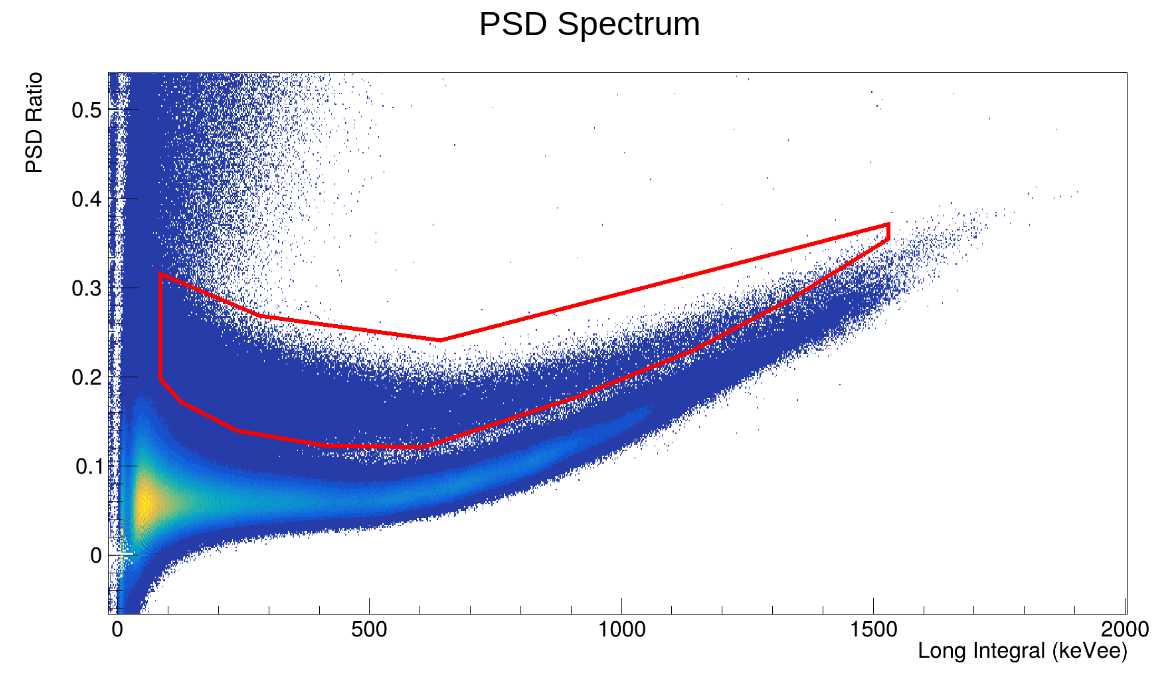
\includegraphics[width=0.6\textwidth]{low_thesh_psd.png}
  \caption{Figure 4.1: PSD spectrum with low threshold.}
  \label{fig:Low Threshold}
\end{figure}

\begin{figure}[h!]
  \centering
  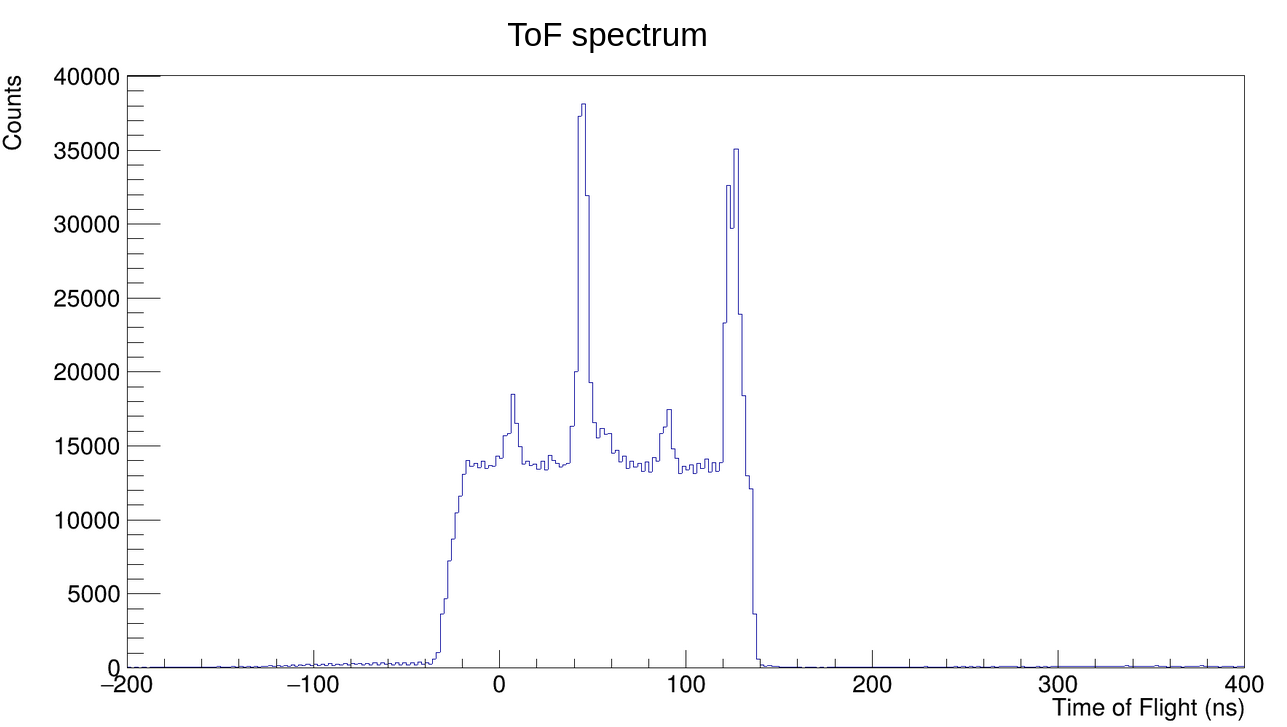
\includegraphics[width=0.6\textwidth]{14o_tof.png}
  \caption{Figure 4.2: ToF spectrum for the $^{12}C(^3He,n)^{14}O$ reaction observed by a CATRiNA detector at 133.5 degrees.}
  \label{fig:14O ToF}
\end{figure}

\begin{figure}[h!]
  \centering
  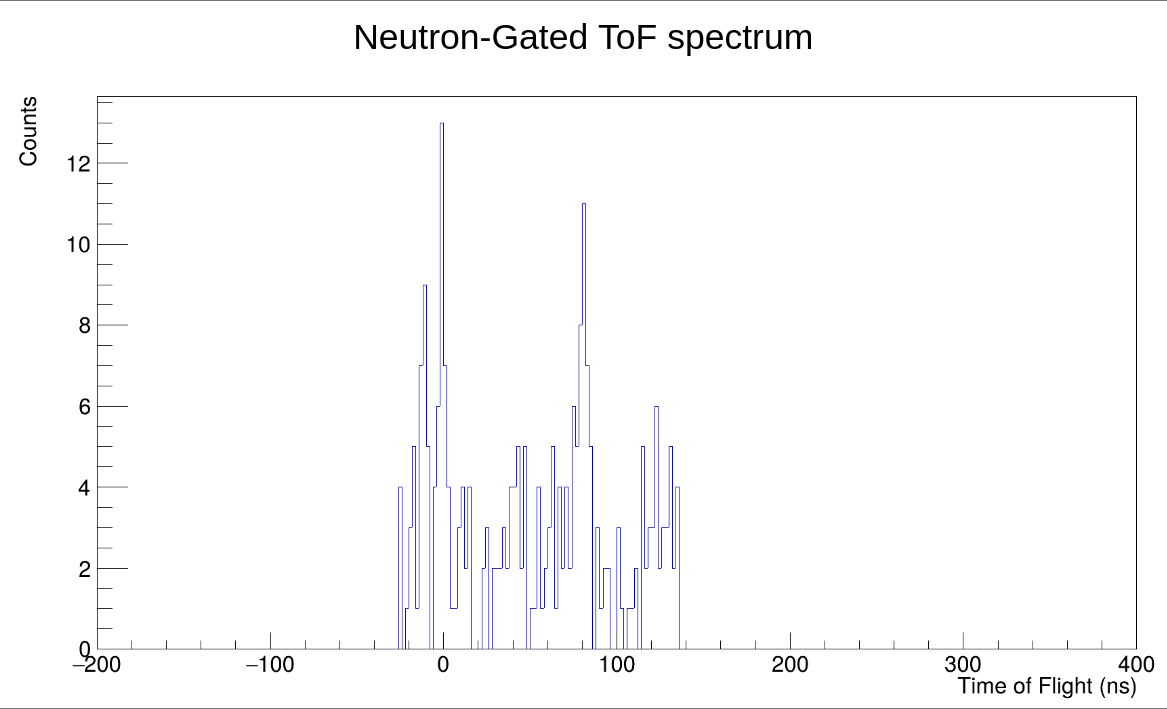
\includegraphics[width=0.6\textwidth]{carbon_gated_tof.png}
  \caption{Figure 4.3: ToFg spectrum.}
  \label{fig:14O ToF Gated}
\end{figure}

\begin{figure}[h!]
  \centering
  \includegraphics[width=0.6\textwidth]{carbon_qval_133.5.png}
  \caption{Figure 4.4: Q-value spectrum.}
  \label{fig:Carbon Q Value}
\end{figure}

\begin{figure}[h!]
  \centering
  \includegraphics[width=0.6\textwidth]{carbon_ex_133.5.png}
  \caption{Figure 4.6: Q-value spectrum.}
  \label{fig:Carbon Excitation}
\end{figure}

The ToF and excitation spectra for the $^{7}Li(^3He,n)^{9}B$ reaction can be seen in the figures below. In Figure 4.7, there are four peaks visible within the ToF spectrum. These peaks arise from gamma radiation from the beam interacting with the target or the beam stop. Prompt gamma emission will occur from various short-lived excitations of the consituent atoms within both locations, resulting in a sharp peak. For this experiment, the coincidence window used in the electronic triggering scheme was widened to 165 ns, allowing for two 82.5 ns RF bunches to be recorded. This results in four peaks, with two peaks per RF bunch. These peaks were identified using the phosphor and the blank targets. The beam only interacts with the phosphor target via luminescence. The blank target allows the beam to pass freely to the beam stop. This results in predicable pairs of peaks in each ToF spectrum that can be compared to the $^{7}Li(^3He,n)^{9}B$ spectrum as a means of peak identification. Once this identification has been carried out, more thorough kinematic reconstructions can be performed. \\ \\

\begin{figure}[h!]
  \centering
  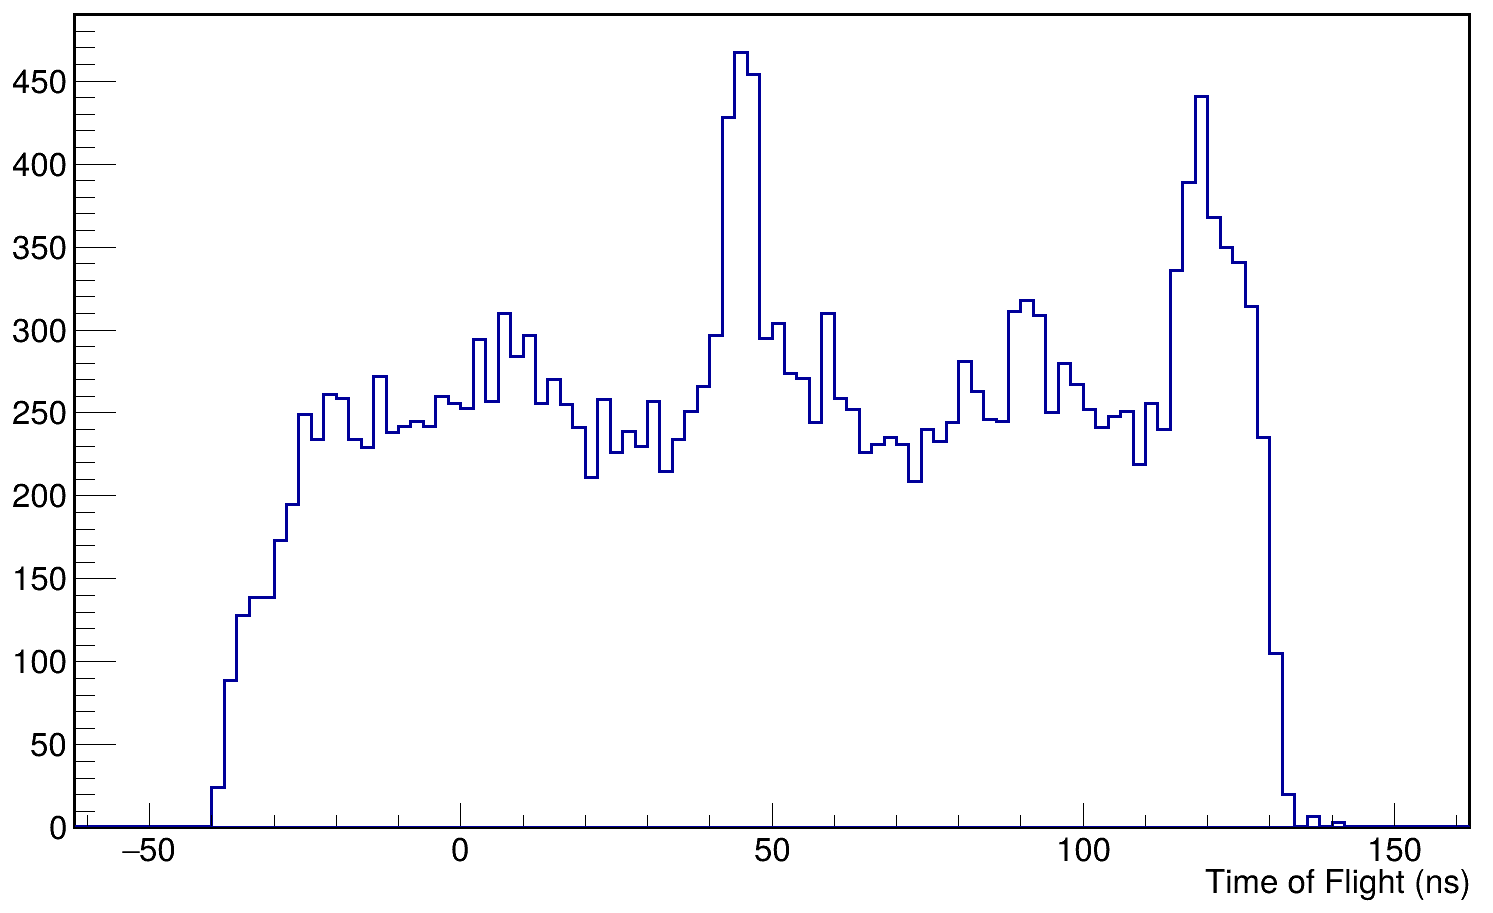
\includegraphics[width=0.6\textwidth]{tof_123.png}
  \caption{Figure 4.7: 7Li tof plot.}
  \label{fig:Li ToF}
\end{figure}

\begin{figure}[h!]
  \centering
  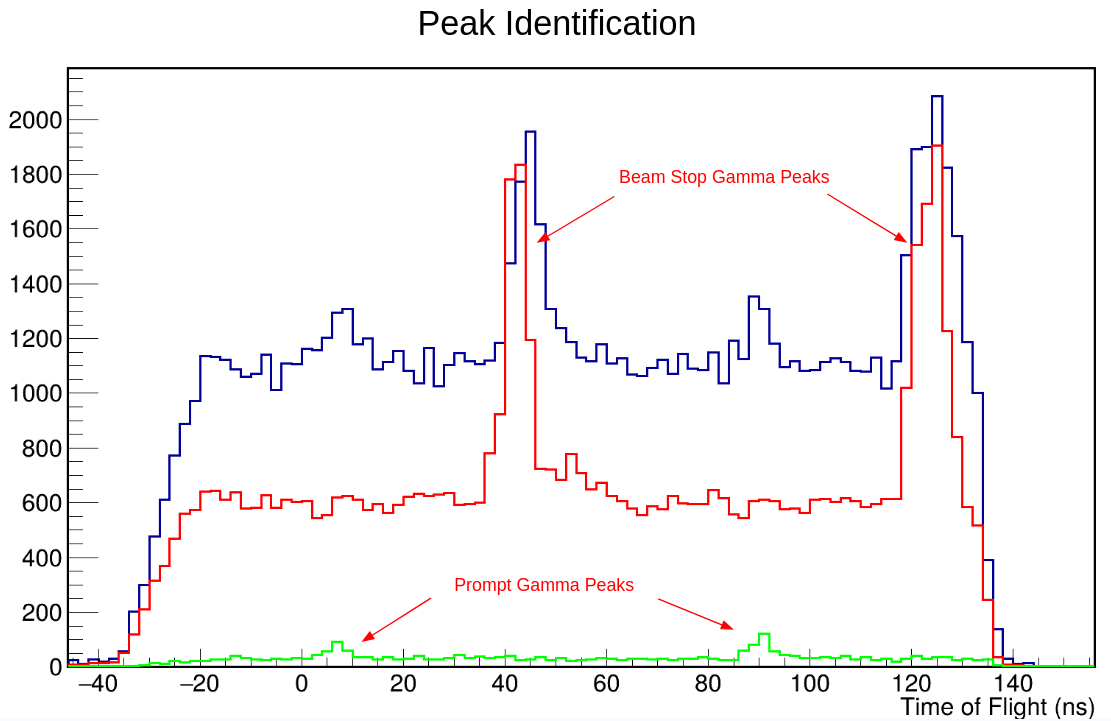
\includegraphics[width=0.6\textwidth]{peak_id.png}
  \caption{Figure 4.8: Comparison of ToF spectra using $^7$Li, $^{12}$C, and phosphor targets. Notice the strength of the gamma peaks populated by beamstop-induced events relative to the peak populated by prompt target reactions.}
  \label{fig:9b Peak Comparison}
\end{figure}

To separate the neutron events from the $\gamma$ events, gates were applied to the PSD spectrum. The PSD spectra are all calibrated in units of keVee. Two threshold values were applied to the PSD spectra. In previous works, a threshold of 55 keVee and 85 keVee was applied to the 2"x2" and 4"x2" detectors. Due to the high beam-stop induced background, our minimum thresholds had to be increased significantly. Excitation spectra were then extracted from the gated events. An excitation spectrum for a detector located at 123 degrees is shown below. 

\begin{figure}[h!]
  \centering
  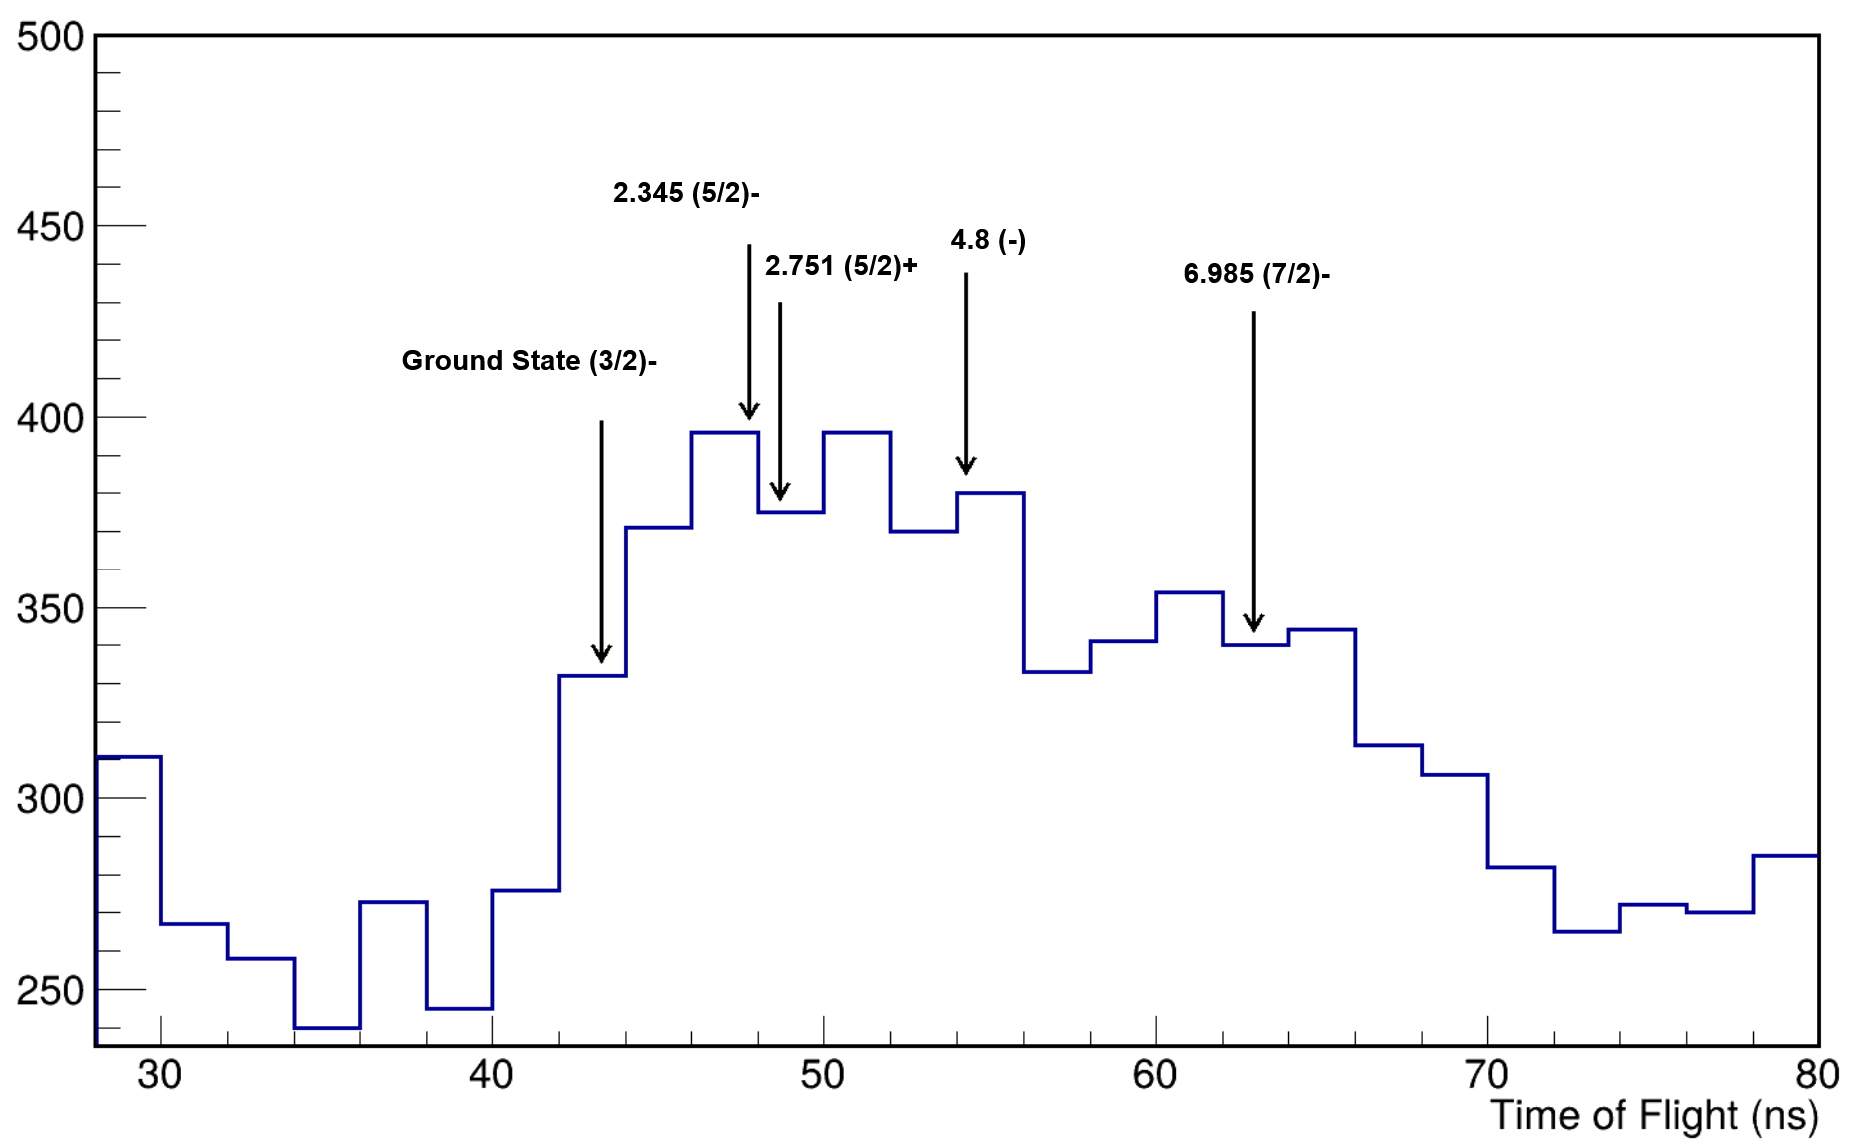
\includegraphics[width=0.6\textwidth]{tof_gated_123_labeled.png}
  \caption{Figure 4.9: A $^7$Li neutron-gated ToF spectrum taken at 123 degrees. The labeled peaks represent expected flight times for neutron groups resulting from a populated state in $^9$B.}
  \label{fig:Gated ToF of 9B}
\end{figure}

\begin{figure}[h!]
  \centering
  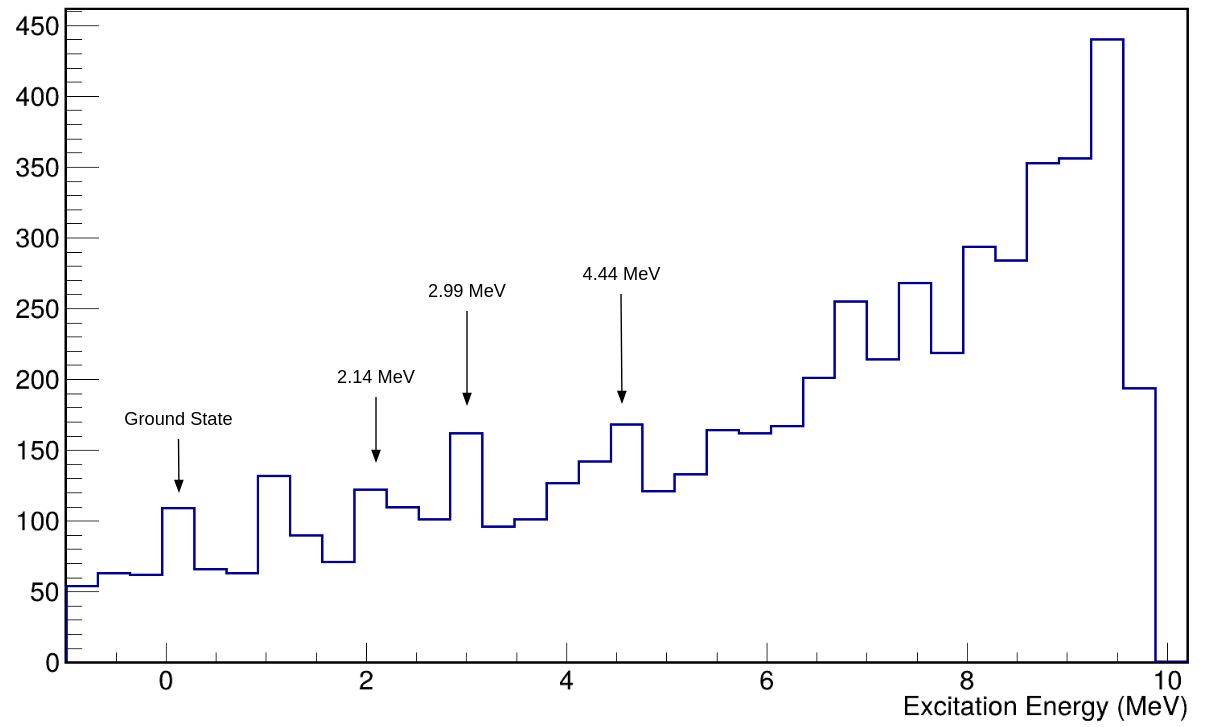
\includegraphics[width=0.6\textwidth]{Excitation_plot.png}
  \caption{Figure 4.10: A $^7$Li excitation spectrum taken at 123 degrees. The labeled peaks represent measured excitation values. It is not clear if the peak between the ground state and the 2.14 MeV peak is the $\frac{1}{2}+$ state.}
  \label{fig:Excitation of 9B}
\end{figure}

In Figure , the expected locations of the highly excited $^9$B states are shown in the spectrum. Due to the low timing resolution, the states are not well-separated within the spectrum. In comparison to previous results found by K. Gul et al. \cite{gul197018o}, the spectra from the current work does not display a prominent ground state peak. However, there appears to be prominent 2.345 and 4.8 MeV peaks within the current spectra. Gul does not list the known 2.751 and 2.78 MeV states separately. In our case, due to poor timing resolution, the two states cannot be separately resolved in this work. A reason the ground state does not display a prominent peak in the ToF spectrum can be attributed to the energy of neutrons within the reaction. Neutrons ejected at 123 degrees from the ground state would have an energy of 10.81 MeV, which indicates that our detectors were not optimized for detecting neutrons at energies greater than 9 MeV. From the excitation spectrum, there appears to be a state in $^9$B with an measured excitation energy of $E_x = 0.12 \pm 0.31$ MeV which is consistent with the known $^9$B ground state width of 0.54 keV. There also appears to be  prominent states at $E_x = 2.14 \pm 0.4$ MeV, $E_x = 2.99 \pm 0.32 MeV$, which is consistent with the known $2.345$ MeV state. There is evidence that the 4.8 MeV state is populated at a measured value of $4.44 \pm 1.1$ MeV, which is consistent with the measured energy and width of the 4.8 MeV state in $^9$B. 

From this work, states in  $^9$B where populated that were consistent with known states found in previous studies. From this dataset, it was not possible to resolve the first excited state of $^9$B. Further work is needed to properly characterize this state using $(^3He,n)$.

\chapter{Future Work}

A more precise measurement was required to characterize this state. A setup that mirrors the previous setup will be employed. A further constraint will be added using a $\Delta E-E$ telescope, which will employ a 65-micron thick S2 silicon detector and a 1001-micron thick S1 silicon detector. This telecscope will be in coincidence with the CATRiNA detectors to measure decay products from the breakup of the $^9$B residual nucleus. Since the charged decay products will deposit different amounts of energy within both silicon detectors, a further PID can be applied to the breakup products of $^9$B, which are listed in the table below. By gating on these breakups for the expected decay energies, the excitation spectra can be further constrained to resolve the states in $^9$B. \\

Future work involves analysis of the upcoming $^7Li(^3He,n)$ reaction using an array of silicon detectors to constrain breakup channels in $^9$B. As of the writing of this prospectus, the analysis is not yet complete.  \\
\\
An experiment to observe highly-excited states in $^9$B will be undertaken, using a higher beam energy, with the goal of precise determination of missing analog states to $^9$Be.
\\ \\

\newpage

\printbibliography

\end{document}
